% Template - https://sanskrit.uohyd.ac.in/18WSC/Style_files/CS_and_DH.tex
\providecommand{\tightlist}{%
  \setlength{\itemsep}{0pt}\setlength{\parskip}{0pt}}

\documentclass[11pt]{article}
\usepackage{scl}
\usepackage{times}
\usepackage{url}
\usepackage{latexsym}
\usepackage{lineno}

\usepackage{fontspec, xunicode, xltxtra}
\newfontfamily\skt[Script=Devanagari]{Sanskrit 2003}
\setmonofont{Sanskrit 2003}


\title{A universal subhāṣita database, and deduplicating sanskrit texts}

\author{Vishvas Vasuki \\
  Dyugaṅgā, Beṅgaḷūru \\
  {\tt https://sanskrit.github.io/groups/dyuganga/}
\\}

\date{}

\begin{document}
\maketitle
%\linenumbers
\begin{abstract}
Subhāṣita-s are popular and beautiful Sanskrit quotations. In this paper, we propose a universal open-source subhāṣita database. As a part of it, we present an algorithm for deduplicating sanskrit texts, as well as one for identifying non-duplicate vairants of a given quote.
\end{abstract}

\section{Motivation}
Subhāṣitas are popular and beautiful Sanskrit quotations - they're usually verses. One of the greatest (and useful) pleasures I've had in tough times is retreat for a while into the world of beautiful Subhāṣitas- so as to burst forth with renewed inspiration and energy. 

Since ages, they have been lovingly compiled [E.g. \cite{subhashita-1952}, \cite{mss-1974}] and memorized. I especially like \textbf{online} collections curated by some friends and myself - since a book is not always available, and I want to collect and easily access choice ones for future enjoyment. But it is tedious (atleast for me) to sit in front of a computer to do the following:

\begin{itemize}
\tightlist
\item
  read them,
\item
  or scour the internet for new ones
\item
  or collect favorites in a spreadsheet
\item
  or just annotate them with comments.
\end{itemize}

So, it is desirable to make the above as simple and easy as possible, and to share our collective labor so that we can benefit more easily from each others' work.

\section{A universal database}

We've set out to build a database of Subhāṣitas - which is:

\begin{itemize}
\tightlist
\item
  \textbf{Universal}

  \begin{itemize}
  \tightlist
  \item
    Its goal is to contain within it every worthy Subhāṣita ever
    composed.
  \item
    In fact, the ultimate ambition encompasses all languages, verse
    and prose forms.
  \end{itemize}

\item
  \textbf{Freely and easily available}.

  \begin{itemize}
  \tightlist
  \item
     Anyone should be able to access it.
  \item
     Anyone should be able to copy and export it to other formats, thereby making it robust to network delays and geopolitical blockage\footnote{For example, unprecedented restrictions - and even ``cancellations" - were imposed on Russian users, sportsmen and artists (both living and long dead) by several Western institutions and internet services in the wake of Western sanctions against Russia around March 2022.}. 
  \item
     Anyone should be able to present it in any way users will find convenient. The data format should be easily parsable in all popular machine languages.
  \item
     Anyone should be able to suggest corrections and annotations. 
  \item
     Maintenance and serving the database should be possible with very low (Ideally 0) budget. 
  \end{itemize}
\item
  \textbf{Growing constantly in number}, thanks to contemporary compositions.
\item
  \textbf{Growing constantly in annotations}, where annotations include ratings, description, translations, metre, flaws, sources \ldots.
\end{itemize}

\section{Implementation}
\subsection{The database}
We have implemented the proposed database as a simple collection of markdown files with TOML metadata. This database available as a Github repository \cite{subhaashita_db_sa_padya}. So, it is version controlled - so that one can view a history of changes made pertaining to any quote. Anyone can suggest additions or other corrections to the database via the well-known mechanism of Github pull requests. Such requests can then be reviewed and accepted by the database maintainers. Furthermore, such repositories are easy to download, clone and rehost as needed. 

As of 19 March 2022, the database consists of about 19k verses - mostly from secondary sources such as \cite{subhashita-1952} and \cite{mss-1974}. Various indices are generated for the convenience of front-end software, so that it is easy to look up all quotations starting with a particular letter, or all quotations pertaining to a certain topic or all Subhāṣitas in a given meter, or all compositions by a given author, or all quotations with a certain rating. Metrical distribution is shown below.

\begin{figure}[h]
\caption{Mechanically deduced metrical distribution}
\centering
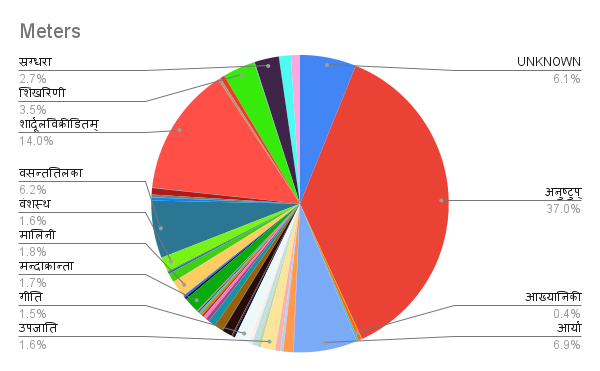
\includegraphics[width=1.0\textwidth]{Meters}
\end{figure}

\subsection{Entry format}
In describing the essentials of the file format we've settled upon, it is best to start with examples. A typical entry, showing two variants of the same verse, is shown below:

\begin{verbatim}
File path: main/A/y/u/S/h/AyuShaHxamaekopisarv_1.md
+++
topics = [ "कालः", "आयुः",]
ratings = [ "vvasuki:5",]
secondary_sources = [ "MSS_5160",]
meters = [ "अनुष्टुप् (श्लोक)",]
jsonClass = "Subhaashita"
title = "आयुषः क्षण"

+++

<details open><summary>Text</summary>

आयुषः क्षण एकोऽपि सर्वरत्नैर्न लभ्यते।  
नीयते यद् वृथा सोऽपि प्रमादः सुमहानयम्॥
__________________
आयुषः क्षण एकोऽपि सर्वरत्नैर्न लभ्यते।  
नीयते स वृथा येन प्रमादः सुमहानहो ॥
</details>

\end{verbatim}

Another example, from the gifted contemporary poet Shankar Rajaraman, recording a note from an unknown source - 

\begin{verbatim}
File path: main/g/a/j/A/m/gajAmamasy.md
+++
topics = [ "गणेशः",]
sources = [ "राजारामज-शङ्करः - मुक्तकम्",]
ratings = [ "vvasuki:5",]
meters = [ "अनुष्टुप् (श्लोक)",]
jsonClass = "Subhaashita"
title = "गजाननस्य जीयासुः"

+++

<details open><summary>Text</summary>

गजाननस्य जीयासुः कर्णतालझलज्झलाः ।  
श्रुत्यन्तवचनैर्यासामनुवादो विधीयते ॥
</details>



<details><summary>अज्ञात-विवरणम्</summary>

श्रुत्यन्तशब्दे श्लेषः।
</details>
\end{verbatim}

\subsubsection{Metadata}
We observe that the \textbf{metadata}, which includes information such as source, secondary source, topic, meter, rating \ldots is recorded in the file header (the section at the top of the file between the two +++ lines). This is stored in TOML \cite{toml} format. It is parsable out of the box by static website generators such as Hugo \cite{Hugo}. The metadata is easily extensible - new fields can be added.

\subsubsection{Text and commentary}
Various versions of the quote and any associated commentaries are stored in HTML detail tags. Within each detail, the content text is stored in the markdown format. The summary tag uniquely identifies this content as belonging to a particular commentary or the quotation text itself. If multiple variants of a Subhāṣita is available, they are recorded one after another, separated by a markdown horizontal rule.

\section{Construction and Maintenance of the database}
Code used for constructing and maintaining the database is available as an open source python package \cite{subhaashita_py}. A critical function of this package is to ensure proper addition or insertion of a new quote or commentary or metadata related to a quote. Particularly, we don't want duplicates in the database, and we want to identify variants easily. Furthermore, we want to automatically update various database indices as needed. This function is called repeatedly when importing quotes from - say - a spreadsheet or a book.

\subsection{Duplicates}
A given pair of sanskrit texts could be duplicates - having an identical set of words, differing only in pronunciation. The following are sources of duplication:

\begin{itemize}
\tightlist
\item
In sanskrit, the very same word can have different forms - for example - {\skt धर्मः} and {\skt धर्म्मः}. If one string of letters can be optionally derived from another using standard grammatical rules, they can be said to represent the same word.

\item
In sanskrit, some euphonic combinations (sandhis) are optional. For example: {\skt तं नय} and {\skt तन्नय}. And, some are not recorded accurately in text even when applied. For example - use of visarga instead of jihvāmūlīya or upadhmānīya.

\item
Sometimes, the text may be presented using the ``lazy anusvāra" orthography. For example: {\skt समितिंजय} for {\skt समितिञ्जय}.
\end{itemize}

\subsubsection{Deduplication}
We tackle the deduplication problem by attempting to reduce each given text to a key which remains the same irrespective of optional forms and orthography. Major steps in this algorithm are the following:

\begin{itemize}
\tightlist
\item
Removal of all non word characters

\item
Replacement of all nasal letters with the letter m

\item
Replacement of all duplicated consonant sequences like {\skt द्द} with just singletons like {\skt द}.
\end{itemize}

The above algorithm is approximate - it identifies duplicates and non-duplicates correctly most of the time. The probability of a mistaken ``duplicate" verdict reduces greatly with the length of the text. This algorithm is implemented as a function (\verb^get_approx_deduplicating_key^) in an open source python library \cite{indic_transliteration_py}. 

We want to apply the above algorithm efficiently. While adding a new subhāṣita, we don't want to have to compare it with each of the 19k items already present in the database (an O(n) operation). Filenames used in our database are based on the deduplicating key described above. So, we just compare with texts from a few select files (an O(1) operation).

\subsection{Variants}
Two non-duplicate quotations are said to be variants of each other if their verbiage differs in such a minor way that the semantic and sonic effect conveyed is roughly the same to the connoisseur. For example, consider the below variants:

\begin{verbatim}
आयुषः क्षण एकोऽपि सर्वरत्नैर्न लभ्यते।  
नीयते यद् वृथा सोऽपि प्रमादः सुमहानयम्॥
__________________
आयुषः क्षण एकोऽपि सर्वरत्नैर्न लभ्यते।  
नीयते स वृथा येन प्रमादः सुमहानहो ॥
\end{verbatim}

While determination of variant can be subjective in some cases (especially in the case of synaesthetic and sensitive connoisseurs), a simple algorithm can help. If the edit distance between two texts is small relative to the text size, the texts are marked as possible variants.

\section{Future work}
Next, we want to develop a good front-end for the database - and - play the pratimāla game on it. We want to enrich the database further - so kind readers are requested to send us typed subhāṣita collections they possess. We also hope that this will motivate other such long-sought-after open-source universal databases for sanskrit (and more generally - literary) connoisseurs, like: one for metres. The front-end clients built for this database could serve as a model for other kāvya readers. Similarly, one can build a collaboratively annotated and rated collection of verses/ sentences within the context of long sequential works (rather than free floating subhāṣitas).

% include your own bib file like this:
\bibliographystyle{acl}
\bibliography{subhashita}
\end{document}